%----------------------------------------------------------------------------------------
%	DOCUMENT CONFIGURATIONS
%----------------------------------------------------------------------------------------

%% Document Setup %%
\documentclass[12pt]{article}
%\usepackage[paper=A4,pagesize]{typearea} % Helps when inserting PDFs
\usepackage[a4paper,margin=3cm,bmargin=3cm,footskip=10mm,headsep=5mm]{geometry}
\usepackage[small]{caption} % Include captions and set default size
\usepackage{fix-cm} % Allows increasing the font size of specific fonts beyond LaTeX default specifications
\setlength{\parindent}{0pt}  % How far to horizontal indent first line of paragraph

%% Fonts %%%
\usepackage{amsmath} % American Mathematical Society Fonts
\usepackage{helvet} % Arial equivilent
\renewcommand{\familydefault}{\sfdefault}

%% Formatting %%
\usepackage{url} % Treat URLs properly
\PassOptionsToPackage{obeyspaces}{url} % Deal with URLs that have spaces in them 
\usepackage{datetime} % Allows custom format of date and time, changes default format of \today
% Below can be removed to have continuous numbers through document, or be modified to subsections etc
\numberwithin{equation}{section} % Set equations to be numbered based on sections
\numberwithin{figure}{section} % Set figures to be numbered based on sections
\numberwithin{table}{section} % Set table to be numbered based on sections

%% Image Set up %%
\usepackage{graphicx}
\usepackage{epstopdf}
\usepackage{wrapfig} % Allow images to be wrapped around rather than having no wrap
\usepackage{float} 	%to allow image to be on the same page
\usepackage{caption}
%\usepackage{subfloat}
\usepackage{subcaption}

%% Lists etc %%%
\usepackage{enumitem}
\usepackage{tabularx}  % Tables where can use X to mean take up all available space
\setlist{nolistsep,leftmargin=*} % Default setup of lists, enumitem etc

%% Extra Sections %%
\usepackage{appendix}  % Allow the ability to have appendix sections
\usepackage[numbers,super,comma,square]{natbib}  % Bibliography Setup, formatting and citations
\bibliographystyle{plainnat}
%\usepackage{footnote} % Can be used for footnotes
%\usepackage[bottom]{footmisc} % Force footnotes to bottom of page

%% Colours %%
%\usepackage[svgnames]{xcolor} % Required to specify font colour
% \usepackage{xcolor} % Required for specifying custom colours

%% Code %%
\usepackage{framed}
\usepackage{listings}
\usepackage{textcomp} % Allows listing code to work without being interpreted as LaTex Code
\usepackage[numbered,useliterate]{mcode} % MATLAB code setup of listings
\definecolor{codebackground}{gray}{0.95}
\lstset{
  language=C,
  basicstyle=\scriptsize\ttfamily, % Ensure consistent font for code
  backgroundcolor=\color{codebackground}, % Set the background color to light grey
  frame=single, % Add a frame around the code
  rulecolor=\color{black}, % Frame color
  breaklines=true, % Break long lines
  literate={~}{$\sim$}{1}, % Handle tilde character
  aboveskip=10pt, % Add vertical space above the listing
  belowskip=10pt % Add vertical space below the listing
} % Set Standard code frame throughout document

%% Misc %%
\newcommand{\hlc}[2][yellow]{ {\sethlcolor{#1} \hl{#2}} } %% Allows the use of \hlc[colour]{text} to get custom highlight
\usepackage[bookmarks]{hyperref} % Allows TOC to be clicked and bookmarks all sections in PDF

%% Custom Title section sizing %%
%\usepackage{titlesec} % Allows custom title properties
%\titleformat*{\section}{\fontsize{10pt}{16pt}\bfseries\raggedright}
%\titleformat*{\subsection}{\fontsize{10pt}{14pt}\raggedright}
%\titleformat*{\subsubsection}{\fontsize{10pt}{14pt}\raggedright}
%\titlespacing*{\section}{0pt}{4mm}{4mm}
%\titlespacing*{\subsection}{0pt}{2mm}{2mm}
%\titlespacing*{\subsubsection}{0pt}{2mm}{2mm}

%------------------------------------------------%
\begin{document}

%----------------------------------------------------------------------------------------
%	TITLE PAGE
%----------------------------------------------------------------------------------------

\pagestyle{empty} 
\vspace*{8cm}
\begin{center}
\Huge
Project Name \\
\vspace{5mm}
\Large
Author \\
\vspace{5mm}
\normalsize
\today
\end{center}

%----------------------------------------------------------------------------------------
%	CONTENT AND FIGURE PAGES
%----------------------------------------------------------------------------------------

\newpage
\pagestyle{plain}
\pagenumbering{roman}
\tableofcontents

%\newpage
%\listoffigures

%----------------------------------------------------------------------------------------
%	CONTENT
%----------------------------------------------------------------------------------------
\newpage
\pagenumbering{arabic}
\pagestyle{plain}
\setcounter{page}{1}

\section{Introduction}

Introduction to Project. Example cite \cite{sigTB} and example references are in appendix \ref{appen:exElements}.\\

\newpage
\section{Design}

How this project is designed to do

\newpage
\section{Implementation}

How the project was implemented \\


\newpage
\section{Conclusion} 

How the project turned out in the end \\


%----------------------------------------------------------------------------------------
% REFERENCES
%----------------------------------------------------------------------------------------
\clearpage
{\raggedright \small
  % The next two lines is so References shows in TOC. If hyperref package enabled,
  %  bookmark will be for prior page
  \let\oldbibsection\bibsection
  \renewcommand{\bibsection}{\oldbibsection\addcontentsline{toc}{section}{References}}
  \bibliography{Bibliography}
}


%----------------------------------------------------------------------------------------
% APPENDICIES
%----------------------------------------------------------------------------------------
\clearpage
\appendixtitleon
\appendixtitletocon
\begin{appendices}
\section{Example Elements}
\label{appen:exElements}


\subsection{Equations}

 Equations with numbers with label \ref{eq:linear_slope}:
\begin{equation}
\label{eq:linear_slope}
 y=mx+c
\end{equation} 


 
Multiline equation (numbered) \\
\begin{equation}
  \label{eq:kinetics}
  \begin{split}
  e(t) &= \omega_{setpoint} - \omega_{feedback} \\
  u &= K_p e(t) + K_d \frac{e(t)}{dt} + K_i \int^{t}_{0} e(t) dt
\end{split}
\end{equation} 

Equation without number 
\[
f(x)=g(\omega)
\]
 
Inline mathematics $u(x)=\delta(x)$ \\
 
Multiline equation (non-numbered) \\
\[
\begin{split}
e(t) &= \omega_{setpoint} - \omega_{feedback} \\
u &= K_p e(t) + K_d \frac{e(t)}{dt} + K_i \int^{t}_{0} e(t) dt
\end{split}
\]


\subsection{Lists}

 \begin{itemize}[leftmargin=1.2cm]
	\item  Item 1
	\item  Item 2
\end{itemize} 
 
 \vspace {10mm}

\colorbox{green}{%
\parbox{\linewidth}{%
%\hlc[green]{
\textbf{To Do Box:}
\begin{itemize}[leftmargin=1cm]
  \item  Task 1
  \item  Task 2
  \item  Task 3
\end{itemize}%
  }%
} % end of colour box
\vspace{5mm}

\subsection{Tables}

Non captioned Tables:
 \begin{table}[htbp]
 \begin{tabularx}{1\linewidth}{ | l || l | X | } 
  \hline 
  Date & Time & Task \\
  \hline 
  7th April 2014 & 2hrs & Project Introduction\\
  1st May 2014 & 2hrs & Final Design Logistics\\
  \hline
\end{tabularx}
\end{table}

Captioned Tables:
\begin{table}[htbp]
 \centering
  \begin{tabularx}{1\linewidth}{ | l || l | X | } 
  \hline 
  Date & Time & Task \\
  \hline 
  7th April 2014 & 2hrs & Project Introduction\\
  1st May 2014 & 2hrs & Final Design Logistics\\
  \hline
  \end{tabularx}
  \caption{Example of a customized captioned tabularx table}
\end{table}
\vspace {10mm}


\subsection{Images}

Auto placed Picture \\
\begin{figure}[ht] 
  \centering
  %\hspace{-7mm}  % Sometimes needed for vector formats
  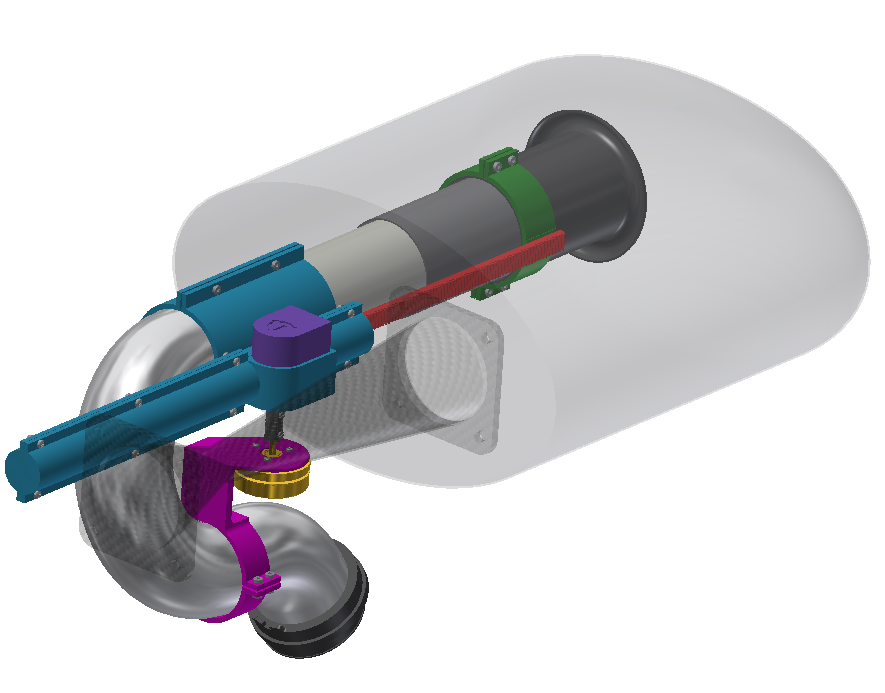
\includegraphics[width=0.5\linewidth] 
      {./figures/example/VLIM.png} 
  \caption{Variable Length Manifold} 
  \label{fig:vlim}
\end{figure}


 
\section{Program Code}
% \lstinputlisting[language=C, basicstyle=\tiny,literate={~}{$\sim$}{1}]{./code/main.c}
Hello World in C (from file)
\lstinputlisting[language=C]{./code/main.c}


Hello World in python (inline)
\begin{lstlisting}[language=python]
print("Hello World")
\end{lstlisting}

\end{appendices}
\end{document}
